\documentclass{jarticle}

\usepackage[ms]{pxchfon}% MSフォントを指定
\usepackage{twocolumn}

%\usepackage[dvi ps]{graphicx} %%画像を読み込む

\usepackage[dvipdfmx]{graphicx} %%画像を読み込む
\newcommand{\setPicture}[1]{\includegraphics[width=1\linewidth]{/Users/watanabe_shouta/2024-chukan/picture/#1}}
  

\usepackage{subfigure}
\usepackage{amsmath}          %%genfrac http://www.biwako.shiga-u.ac.jp/sensei/kumazawa/tex/form006.html
%\usepackage{newtxtext,newtxmath}
\usepackage{ulem}             %%http://biwako.shiga-u.ac.jp/sensei/kumazawa/tex/ulem.html     uline,uuline,uwave,sout,xoutなど
\usepackage{multirow}
\usepackage{chukan2020}       %%最後に読み込むこと!(最後に読み込まないと\textwidthなどの設定が反映されない)

\pagestyle{empty} %ページ番号を入れるときにはコメントアウトする

\begin{document}

\linesparpage{50}

\title{
柔軟な/屈曲可能な胴体を有する魚型ロボットの開発
}
\etitle{
 Development of Fish-Type Robot with Flexible/Bendable Torso
}
\author{
研究者 渡部 翔太\;\;\;
指導教員 中西 大輔
}
\eauthor{
Keywords: Fish-Type Robot, Flexible/Bendable Torso
}

\maketitle

\thispagestyle{empty}  %1ページ目にページ番号を入れるときにはコメントアウトする

%%%%%%%%%%%%%%%%%%%%%%%%%%%%%%%%%%%%%%%%%%%%%%%%%%%%%%%%%%%%%%%%%%%%%%%%%%%%%%%
\section{はじめに}

水中・水上の推進システムには船舶によく見られるスクリュープロペラを用いた推進方法や,魚を模したロボットによる尾びれ推進などがあげられる.
スクリュープロペラは推進性能が高く,広く船舶などに用いられてきた.その一方で,スクリューは周辺環境への影響が大きく,水棲生物の生態系の調
査や災害への支援に用いられる推進システムとして適していない.それに対して,尾びれ推進は周辺環境へ影響を与えず,加速性・旋回性に優れている.
こういった点から尾びれ推進を用いた魚型ロボットの開発は生態系調査や災害への支援といった面において注目されている.

これに対して先行研究では,飛び移り座屈を用いた魚型ロボットやワイヤ駆動式の魚型ロボットが開発されてきた.

%%%%%%%%%%%%%%%%%%%%%%%%%%%%%%%%%%%%%%%%%%%%%%%%%%%%%%%%%%%%%%%%%%%%%%%%%%%%%%%
\vspace*{-2mm}
\section{デッドコピーの作成}
\subsection{コピー元の選定}
今回,研究を進めるにあたってまずは昨年度の研究で開発された魚ロボットのデッドコピーを作成することにした.デッドコピーとは既存の工業製品や商品などの構造・使用を
完全に,もしくはほとんどの部分で踏襲して複製した模造品のことである.
今回は魚らしい動きの実現のためにワイヤ駆動型魚型ロボットをコピー元とした.
シミュレーション実験を行う際には,Cyberbotics社のロボットシミュレータソフトウェアWebotsを使用する.
犬型ロボットのシミュレーションモデルには実機ロボットを参考に構築されたモ
デルを使用する.

\begin{figure}[!b]
  \begin{center}
   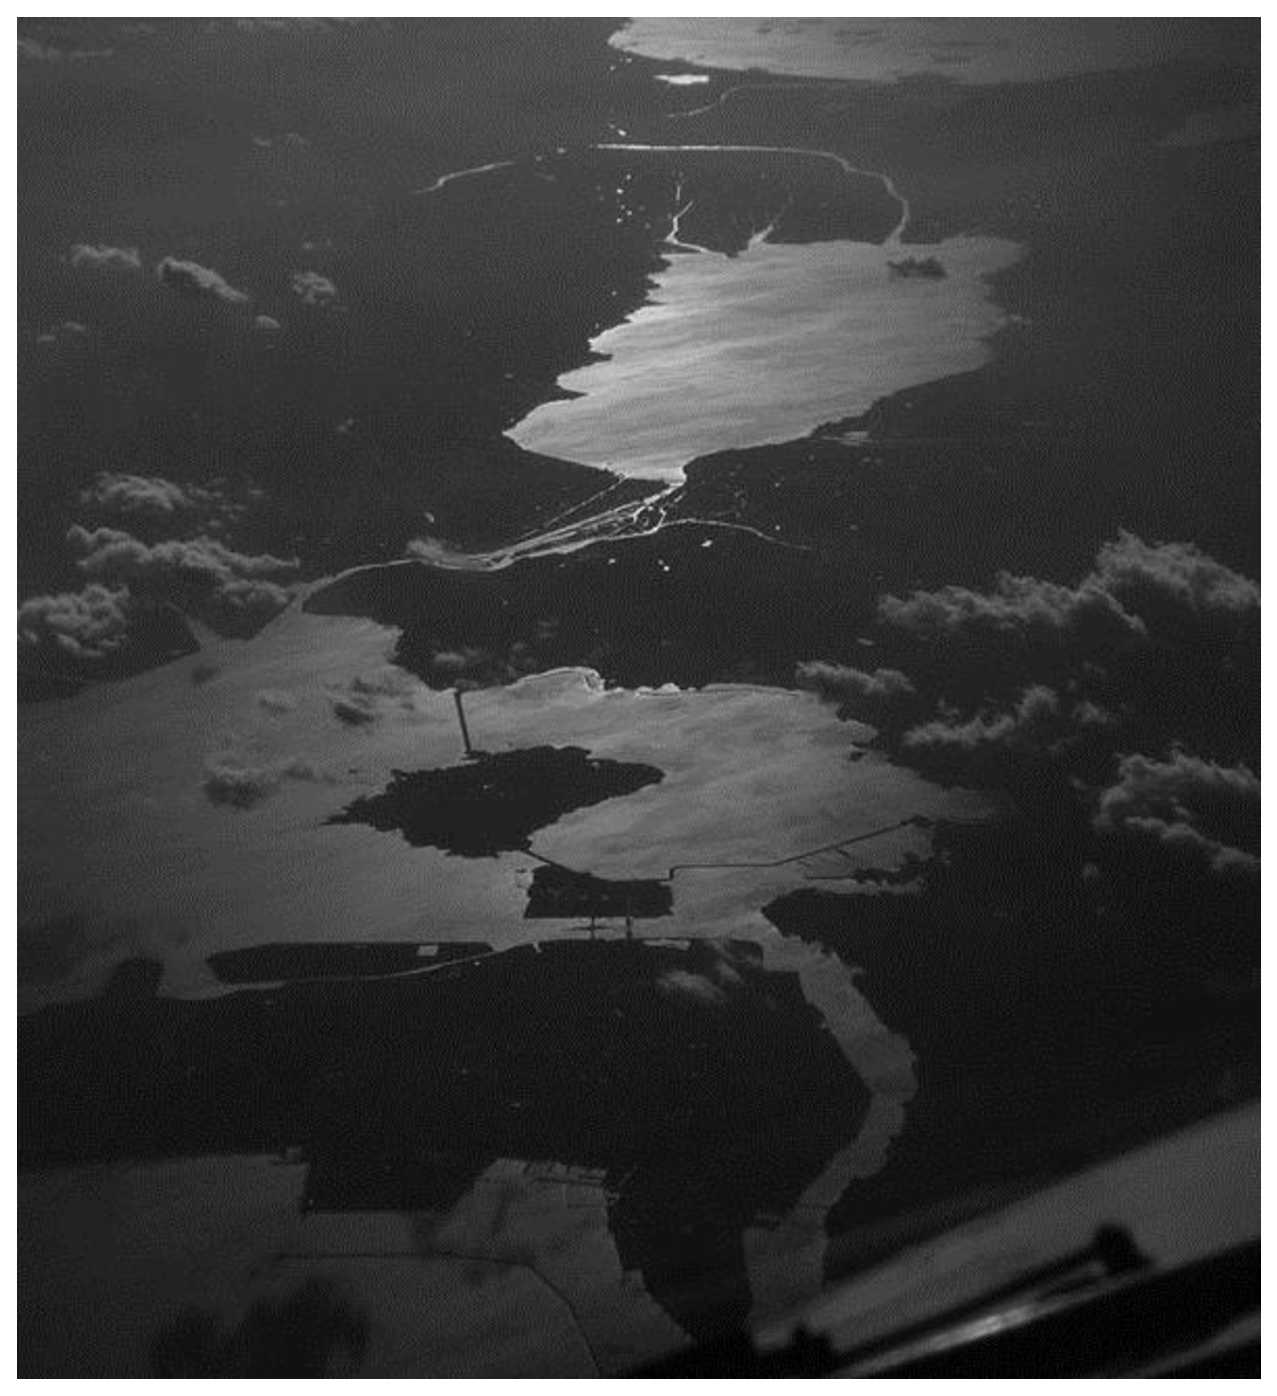
\includegraphics[height=33mm,width=70mm]{Fig/Fig1.eps}
   \vspace*{-4mm}
   \caption{図面の例}
   \label{robot}
  \end{center}
\end{figure}

%%%%%%%%%%%%%%%%%%%%%%%%%%%%%%%%%%%%%%%%%%%%%%%%%%%%%%%%%%%%%%%%%%%%%%%%%%%%%%%
\vspace*{-2mm}
\section{まとめと今後の予定}

卒業研究では,犬型ロボットに強化学習を適用し,特定の初期状態から起き上がり動作を獲得することを実現した.現在,任意の初期状態での起き上がり動作の獲得の方法について検討を行っている.
まず,犬型ロボットの歩行時の転倒パターンのデータを収集した.それらをもとに,主成分分析を用いて,ロボットの転倒パターンの分布を調べ,大まかに3つのパターンに分けられることを確認した.
また,パターンAの犬型ロボットが横転している状態から起き上がる動作を人間がプログラミングすることにより,実際にロボットが起き上がることができることを確認した.

今後の予定として,横転した状態(パターンA)からパターンCに至る動作の獲得を強化学習により実現する.
パターンCから起き上がる動作は卒業研究で獲得済みであるため,最終的に横転した状態からの起き上がりが可能となる.

%%%%%%%%%%%%%%%%%%%%%%%%%%%%%%%%%%%%%%%%%%%%%%%%%%%%%%%%%%%%%%%%%%%%%%%%%%%%%%%
\begin{thebibliography}{99}

\bibitem{Horiuchi2013}
堀内 匡,
NGnetを用いた強化学習によるロボットの行動獲得,
電気学会技術報告「機械学習技術の基礎と応用」,pp.23-27, 2013

\bibitem{Ishikura2014}
石倉裕貴,岸本良一,堀内 匡,
CPGと強化学習を用いた多脚ロボットの行動獲得に関する検討,
電気学会研究会資料,システム研究会ST-13-120, pp.25-28, 2013

\bibitem{Nagami2014}
永海 昂,堀内 匡,
強化学習を用いた四脚ロボットの起き上がり動作の獲得に関する検討,
平成26年電気学会電子・情報・システム部門大会講演論文集,pp.1763-1764,2014

\end{thebibliography}
\end{document}